\section{Methodology}\label{sec:methodology}

\subsection{Application as Finite State Machine with centralized state}\label{sec:central_state}

Development of the project focused on an individuation of a hierarchical Javascript object structure that allow to fully represent all the parts that there are on a plan. The application state is described with an \textbf{immutable tree structure} of which is maintained a reference of the root node. Each atomic change require: (i) The build of a new state \texttt{s'} equal to the previous state \texttt{s}; (ii) Execution of changes on the new state \texttt{s'}; (iii) A replace of the root reference from \texttt{s} to \texttt{s'}. From the memory point this operations would require a lot of resource. To avoid this problem the implementation \textbf{Immutable.js}~\footnote{https://facebook.github.io/immutable-js/} made by Facebook, simulate immutability pattern, avoiding the deep clone of the memory.

The centralized state handling allow to develop features that have as unique goals the creation of a new state coerent with the requested change, without to manage on UI or any other component. The UI adjustment to the new state works thatk to some mechanisms that we will illustrate in the section~\ref{sec:ui_components}.

Thanks to the history of each state generated to the application and thanks to guarantees offered by the immutability pattern we can, in each moment, perform a redo operation to an oldest state, by means of a replace of the current state with one from any of the past state.

To dominate the complexity of the application the system is modelled on a state machine. Thanks to a model based on actions and reducer offered by the pattern \textbf{unidirectional data flow} we have found a directed graph the show all available evolutions of the application state. Each node correspond to a \textbf{mode}, each edge correspond to an action that the user can execute starting from a node. Depending on the mode each event browser, for example \texttt{click} or \texttt{mousemove}, is mapped on an action. A part of the state machine is shown in figure~\ref{fig_uc_draw_wall}.

Centralized state handling and the logic handling by mean of a state machine modelling has been possible thank to the library \textbf{Redux.js}~\footnote{http://redux.js.org/}.


\begin{figure}[!t]
\centering
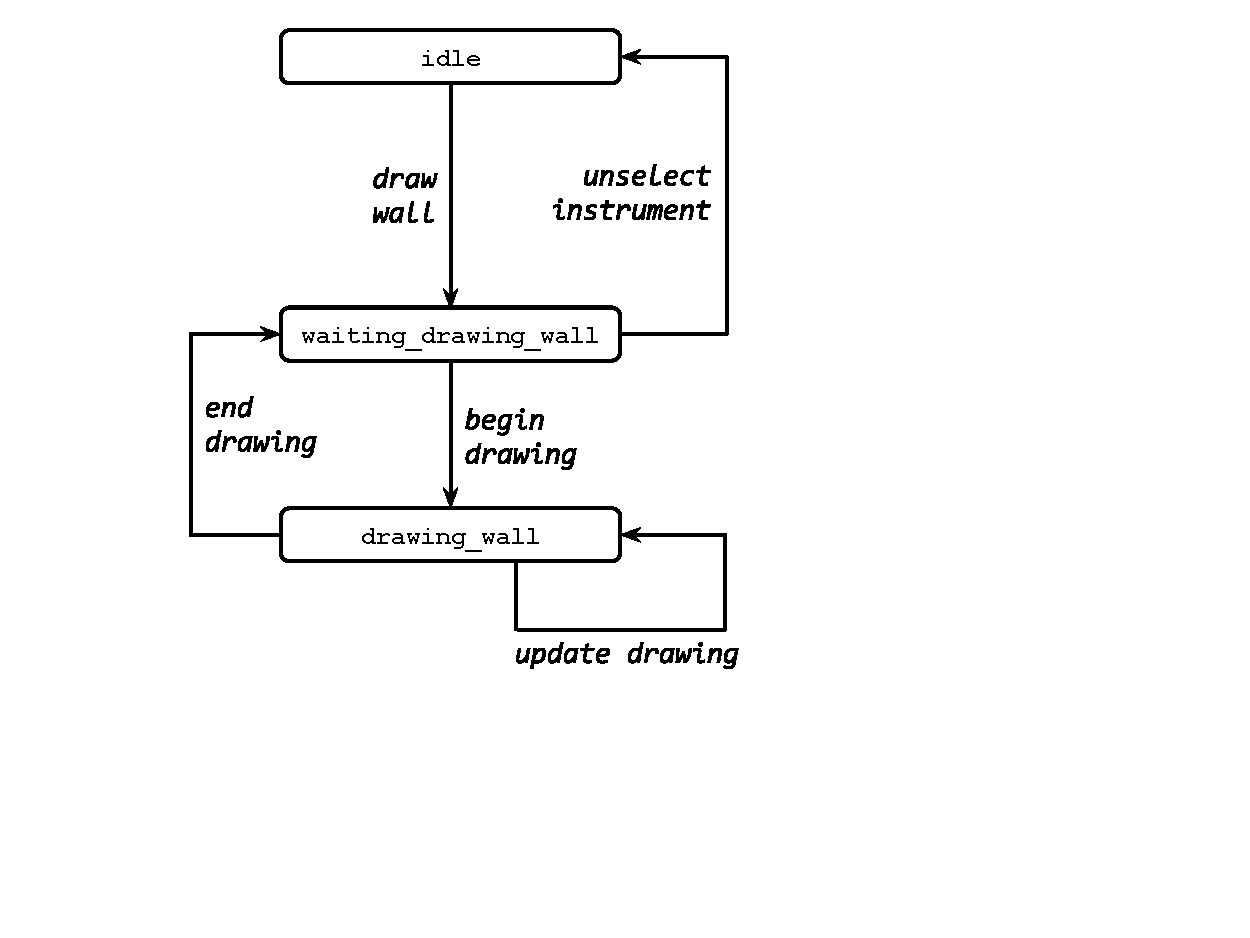
\includegraphics[width=0.6\linewidth]{contents/images/uc_draw_wall}

\caption{Subgraph of the state machine that show a wall creation. (i) Node \texttt{idle}: waiting mode of the application. No action has yet been taken. (ii) Node \texttt{waiting\_drawing\_wall}: user has selected wall design tool, but he hasn't already started the draw phase. (iii) Node \texttt{drawing\_wall}: user has placed the starting point of the wall.}
\label{fig_uc_draw_wall}
\end{figure}


Lo sviluppo del progetto si \`e focalizzato sull'individuazione di una struttura gerarchica di oggetti Javascript in grado di rappresentare in modo esaustivo l'insieme delle componenti presenti sulla planimetria. L'intero stato dell'applicazione viene descritto da una \textbf{struttura ad albero immutabile} di cui viene mantenuto un riferimento al nodo radice. Ciascuna modifica atomica corporta: (i) La creazione di un nuovo stato \texttt{s'} identico al precedente stato \texttt{s}; (ii) L'applicazione delle modifiche allo stato \texttt{s'}; (iii) La modifica del puntatore che rappresenta lo stato corrente da \texttt{s} ad \texttt{s'}. Dal punto di vista della gestione della memoria questo meccanismo richiederebbe un importante dispendio di risorse. Per evitare ci\`o l'implementazione \textbf{Immutable.js}~\footnote{https://facebook.github.io/immutable-js/} realizzata da Facebook, adotta dei meccanismi che simulano il principio di immutabilit\`a evitando la copia in profondit\`a della memoria  (deep clone).

La gestione centralizzata dello stato permette lo sviluppo di funzionalità che hanno come unico obiettivo la creazione di un nuovo stato coerente con la modifica richiesta, senza la necessità di agire sull'interfaccia o su qualsiasi altro componente in esecuzione. L'adeguamento dell'interfaccia grafica al nuovo stato viene effettuato secondo i meccanismi descritti nella sezione~\ref{sec:ui_components}.

Memorizzando la storia di tutti gli stati generati dall'applicazione e sfruttando le garanzie offerte dall'immutabilità si può effettuare, in qualsiasi momento, un'operazione di redo ad un vecchio stato attraverso la sostituzione dello stato corrente con uno qualsiasi tra quelli passati.

Per dominare la complessit\`a dell'applicazione l'intero sistema \`e stato modellato su una macchina a stati. Sfruttando il modello basato su azioni e reducer messo a disposizione dal \textbf{pattern unidirectional data flow} \`e stato individuato un grafo che rappresenta le possibili evoluzioni dello stato dell'applicazione. Ogni nodo corrisponde ad una \textbf{modalit\`a}, ogni arco corrisponde alle possibili azioni che è possibile intraprendere a partire da quel punto. A seconda della modalit\`a gli eventi del browser, come ad esempio \texttt{click} o \texttt{mousemove}, vengono mappati sulle azioni. Un estratto della macchina a stati \`e presente in figura~\ref{fig_uc_draw_wall}.

La gestione dello stato centralizzato e la gestione della logica applicata realizzata  attraverso la modellazione di una macchina a stati è stata possibile sfruttando l'implementazione messa a disposizione dalla libreria \textbf{Redux.js}~\footnote{http://redux.js.org/}.


\begin{figure}[!t]
\centering
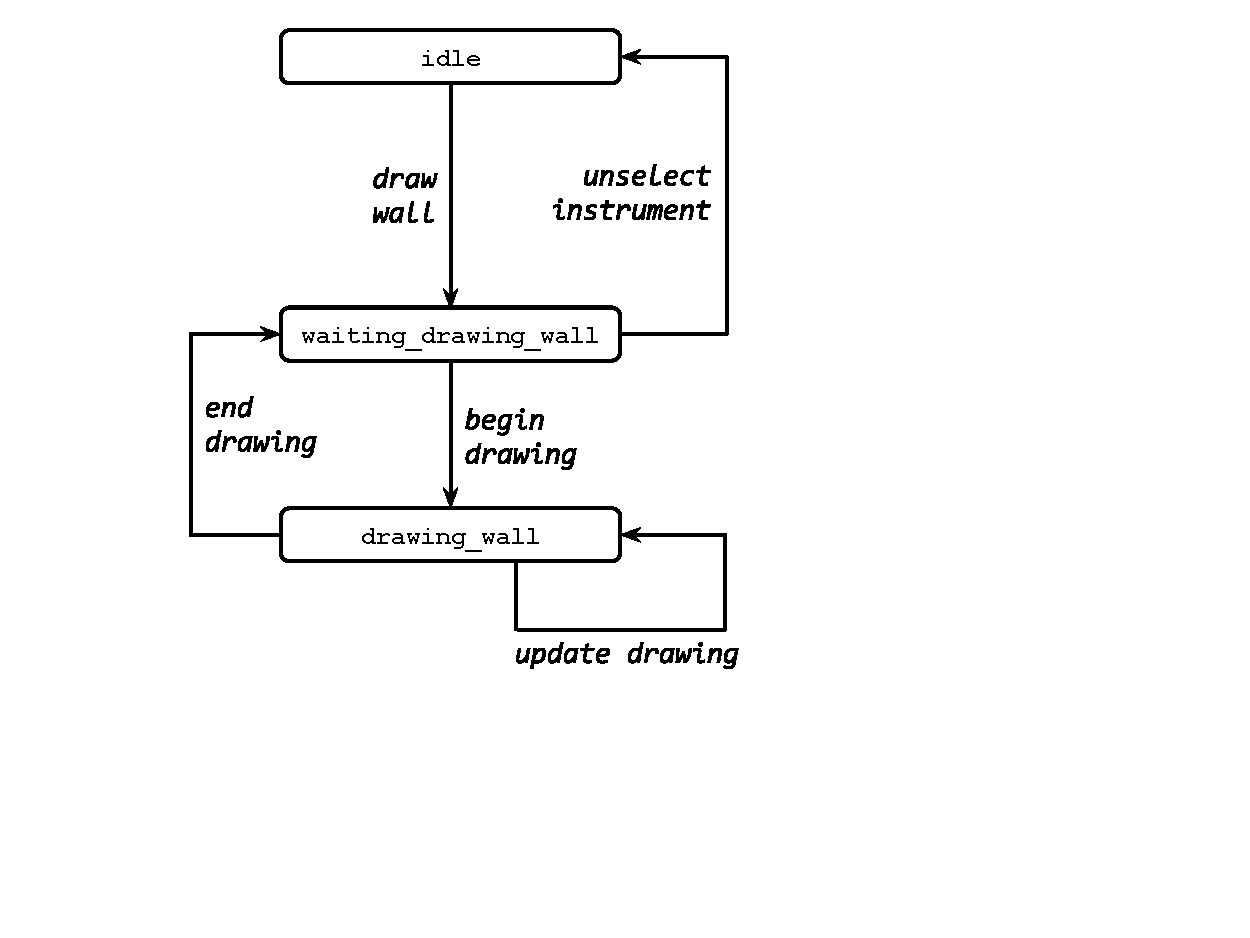
\includegraphics[width=0.6\linewidth]{contents/images/uc_draw_wall}

\caption{Sottografo della macchina a stati che rappresenta la creazione di un muro. (i) Nodo \texttt{idle}: modalit\'a d'attesa dell'applicazione. Non è stata ancora intrapresa nessuna operazione. (ii) Nodo \texttt{waiting\_drawing\_wall}: l'utente ha selezionato lo strumento disegno muro, ma non ha ancora iniziato il disegno. (iii) Nodo \texttt{drawing\_wall}: l'utente ha posizionato il punto di inizio del muro.}
\label{fig_uc_draw_wall}
\end{figure}


\subsection{Collaboration}


Now we will study the mechanisms chosen to provide collaboration for the same project, among users on different PCs. In literature there are many techniques for introducing collaboration between remote users. For example in~\cite{Ellis:1989:CCG:66926.66963} we can find the \textbf{Operational Transformation} technology, where a group of nodes exchanges messages without a \textit{central control point}. It is based on two main properties: (i) you can transform changes relative to other changes and (ii) there is no matter in which order concurrent changes are applied, you end up with the same document.\\

However, the adoption of the uniflow pattern, with a global state, had suggested us to use another methodology for the collaboration feature. Following the principles of these patterns, the application is based upon a \textbf{centralized topology} for communication between nodes. With this approach the state is shared between several instances of the application with a communication infrastructure for the synchronization with the nodes. With this kind of topology, we avoided the peer-to-peer synchronization routines to remove implementation problems regarding the network infrastructure (for example ones caused by the \textit{Network Address Translation}) common when using these kind of systems. Anyhow, this approach it does not influence the serverless nature of the architecture, as the communication systems are external (we adopted \textbf{Firebase}\footnote{https://firebase.google.com/} for the data exchange between users)


\subsection{Building elements}\label{building_elements}

Each building element that the user can add on a plan is available thought a \textbf{catalog}, structured in categories. Each category identify a group of use case whereby the user can interact.\\\\
  \textbf{Walls}, each kind of wall (perimetral, interior, structural) is part of this category. The user can add a new wall selecting the begin and end of the element. The internal state of all the walls correspond to an undirected graph: each \textbf{node} match geometric points in which are intersected more walls and has a couple of coordinates that place it on a 2D space; each \textbf{edge} match a specific wall.
  This internal rappresentation offer a good interactive level to drag and drop walls operations: each wall drag is performed by means of a relocation of a node that cause, other that the displacement of the requested wall, a displacement of each adiacent wall.\\\\

  \textbf{Openings}, each element that hole a wall (windows, doors, arches) is part of this category. The user can add a new opening thanks to a snap on an existent wall. The internal state link each element with its wall.

   \textbf{Areas}, floor belong to this category. They are automatically generated thank to a wall graph analysis. The algorithm is composed of few phases: (i) Search of biconnected component by mean of Hopcroft-Tarjan algorithm~(see \cite{Hopcroft:1973:AEA:362248.362272}); (ii) Removal of edges that are not part of a biconnected component; (iii) Search of all cycles through an algorithm that do a double check of each edges sorted by angle; (iv) Search of maximal cycles correspondent to perimeter edges by an application of Gauss's area formula [CITAZIONE????????]; (v) Removal of maximal cycles;

   \textbf{Objects}, each element that can be arranged on an area is part of this category. The user can interact with the object and change its disposal and rotation.

L'insieme degli elementi che \`e possibile inserire all'interno della planimetria vengono gestiti in un \textbf{catalogo}, strutturato in categorie.
La categorizzazione individua un insieme di casi d'uso con cui l'utente pu\`o interagire.\\\\
\textbf{Walls}, rientrano in questa categoria tutti i tipi di muro (perimetrali, interni, portanti). La creazione avviene specificando il punto di inizio e fine dell'elemento. La rappresentazione interna viene ricondotta a quella di un grafo in cui: i \textbf{nodi} corrispondono ai punti geometrici in cui si intersecano pi\`u muri e hanno delle coordinate che li collocano nello spazio; gli \textbf{archi} corrispondono al muro. Questa rappresentazione garantisce inoltre un’efficace risposta alle operazioni di drag and drop sui muri: ogni spostamento viene applicato attraverso la modifica della posizione dei nodi comportando, oltre allo spostamento del muro richiesto, un riposizionamento di tutti i muri adiacenti.\\\\
\textbf{Openings}, rientrano in questa categoria gli elementi che bucano i muri come porte, finestre e archi. La creazione viene effettuata attraverso uno snap sui muri precedentemente creati. La rappresentazione interna associa ciascuna apertura con il muro di riferimento, creando un legame tra le due componenti.\\\\
\textbf{Areas}, rientrano in questa categoria i pavimenti. La creazione viene effettuata automaticamente attraverso un'analisi del grafo composto dai muri. L'algoritmo individuato si compone delle seguenti fasi: (i) Ricerca delle componenti biconnesse attraverso l'applicazione dell'algoritmo Hopcroft-Tarjan~(vedi \cite{Hopcroft:1973:AEA:362248.362272}); 
(ii) Rimozione degli archi che non appartengono alle componenti biconnesse; 
(iii) Individuazione di tutti i cicli attraverso una doppia visita degli archi ordinata rispetto ad un angolo;
(iv) Individuazione dei cicli massimali, corrispondenti ai cicli che coinvolgono tutti gli archi perimetrali del grafo attraverso la Gauss's area formula;
(v) Rimozione dei cicli massimali.\\\\
\textbf{Objects}, rientrano in questa categoria tutti gli oggetti posizionabili sulle aree. L'utente pu\`o agire sulla disposizione sia in termini di posizione che rotazione.\\

\subsection{UI components}\label{sec:ui_components}

The entire application has been developed using separated modules, following the \textbf{SOLID programming} principles, as it could be expanded. For the web part, we have used the \textbf{web components pattern}, with the implementation of \textbf{React.js}\footnote{https://github.com/facebook/react} written by Facebook. The main idea is to define the frontend application as a collection of components, each one rendered in a different way according with values assigned to the state. In Figure~\ref{fig_ui} we have an example of based on our application.\\

\begin{figure}[h]
\centering
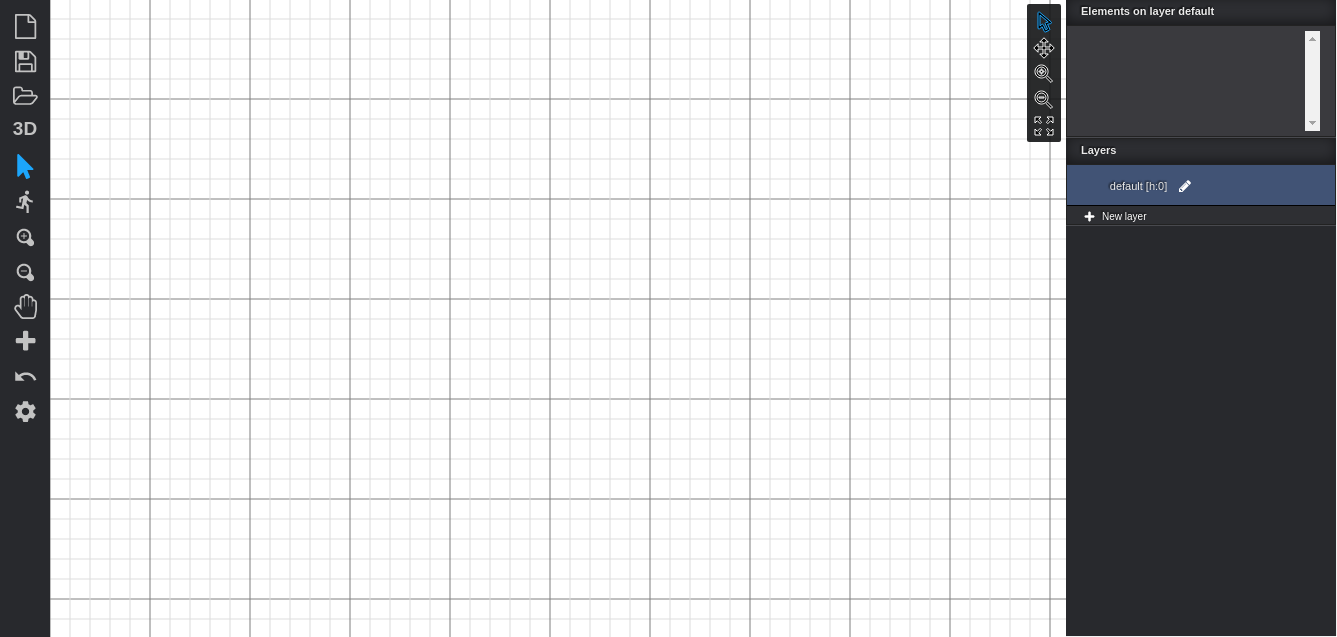
\includegraphics[width=0.65\linewidth]{contents/images/ui}\\
\caption{The user interface of the application with the most interesting components: the toolbar (where every button is another component), the sidebar and the 2D viewer}
\label{fig_ui}
\end{figure}

In particular, the most interesting components developed by us are the \textbf{viewers}, for example the 2D-viewer and the 3D-viewer. This component-based structure, allows us to define whatever state definition (for example in a tabular form) simply adding a new component.\\

The viewers structure is outlined in figure~\ref{fig_viewers}, where we can observe the great blocks. The first one is the \textit{catalog} and as we have already seen in section~\ref{building_elements} it contains all the building elements with their properties. We also the the application \textit{core}, which manages the state and contains all drawing functionalities. It communicates with the catalog taking the building models properties. At least we have the \textit{viewers}, that are chosen observing the current state mode (see section~\ref{sec:central_state}). At the moment we implemented the 2D and 3D viewers (see figure~\ref{fig_viewer})\\\\
\textbf{2D Viewer}. This viewer creates a 2D view of the building model. Given the state, it exploit the \textbf{Virtual DOM} (see~\cite{vdom}) implemented by React.js, to update only changed parts avoiding continuously global updates.\\\\
\textbf{3D Viewer}. It exploits the WEBGL-based modeling library \textbf{Three.js}~\footnote{https://threejs.org/} to build a 3D view of our building. To avoid global refreshes every time we update a part of the state, it has been implemented a \texttt{diff} and \textit{patch} system standardized in~\cite{rfc6902}. So it has been implemented a data structure which maps the Three.js objects with the building elements inside the state. Every time the user launches a Redux.js action, the application compute the difference between the old state and the new one a redraw only the changed objects. In particular we can have the following \textit{operations}: (i) \textbf{add}, (ii) \textbf{replace} and (iii) \textbf{remove}. For every operation it is determined a behavior based on the changed building element, changing also related building elements.

\begin{figure}[htb]
\centering
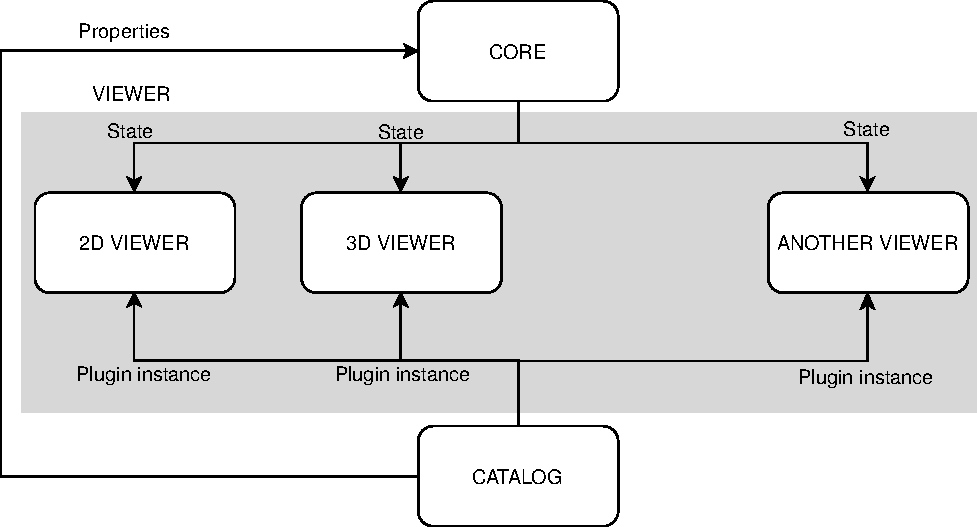
\includegraphics[width=\linewidth]{contents/images/diagramma-visualizzatori}

\caption{The architectural schema for the viewers. Here we can see that the core can instantiate several different viewers giving them the state for the representation}
\label{fig_viewers}
\end{figure}

\begin{figure}[htb]
\centering
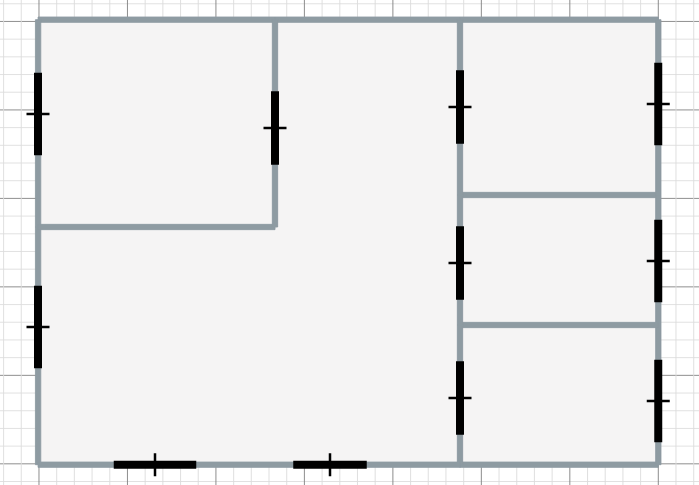
\includegraphics[width=0.45\linewidth]{contents/images/2d-viewer}
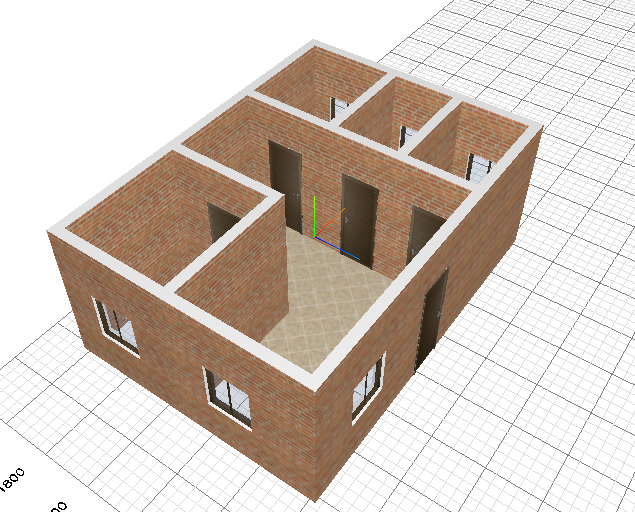
\includegraphics[width=0.45\linewidth]{contents/images/3d-viewer}
\caption{The 2D and 3D viewers for the state}
\label{fig_viewer}
\end{figure}

\subsection{Architettura serverless}
Una tra le sfide che ha caratterizzato il progetto \`e l'utilizzo di un approccio serverless. L'intera applicazione viene eseguita all'interno del browser, ottenendo i vantaggi di: (i) evitare all'utilizzatore complicate installazioni del sistema o procedure di aggiornamento; (ii) fornire un livello di astrazione tale da rendere l'ambiente compatibile su diverse macchine e su diversi sistemi operativi; (iii) abilitare un rilascio di nuove versioni centralizzato, in grado di raggiungere tutti gli utenti contemporanemante; (iv) eliminare il punto di concentramento del calcolo in quanto questo rimane confinato sulla macchina dell'utente.
Per permettere la generazione di elementi architetturali complessi il sistema \`e in grado inoltre di sfruttare dei worker di tipo FaaS (Function as a Service) demandando l'onerosa generazione delle geometrie 3D necessarie alla visualizzazione. Nella figura~\ref{fig_serverless} c'\`e uno schema dell'architettura dell'applicazione
\begin{figure}[htb]
\centering
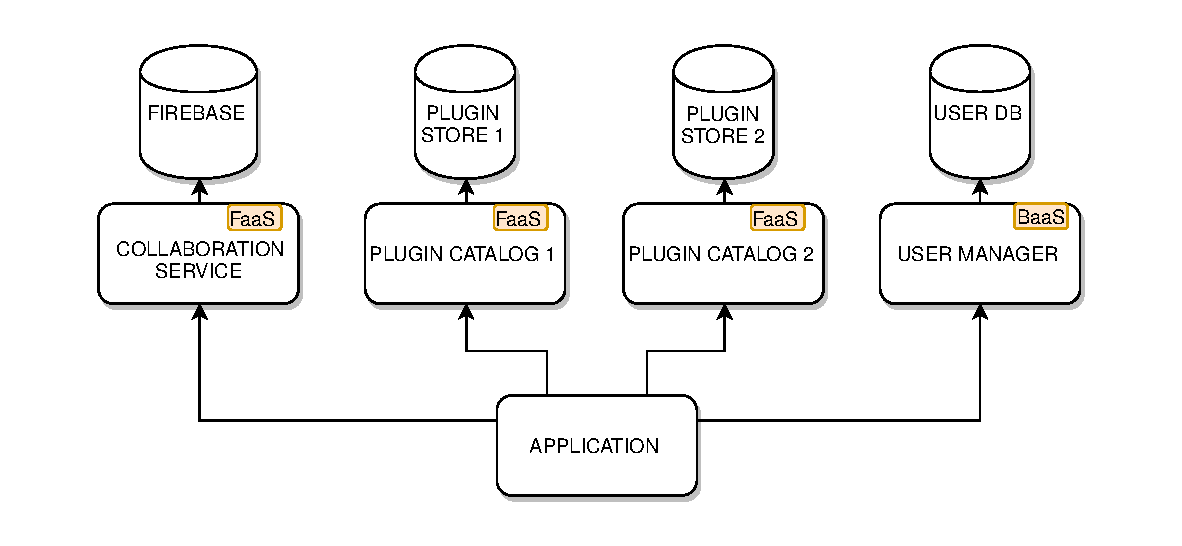
\includegraphics[width=\linewidth]{contents/images/serverless-diagram}

\caption{The serverless architecture for our application. We can recognize the collaboration component, based on Firebase. We can also see the FAAS container for the plugin catalog which is linked with a BAAS component for plugins generated on server with other modeling software. We can also manage an optional user login to the system, with another BAAS. Notice that the core application is entirely run on front end side}
\label{fig_serverless}
\end{figure}